 % SIAM Article Template
\documentclass[review,onefignum,onetabnum]{siamart171218}

% Information that is shared between the article and the supplement
% (title and author information, macros, packages, etc.) goes into
% ex_shared.tex. If there is no supplement, this file can be included
% directly.


% Packages and macros go here
\usepackage{lipsum}
\usepackage{amsfonts}
\usepackage{graphicx}
\usepackage{epstopdf}
\usepackage{algorithmic}
\ifpdf
  \DeclareGraphicsExtensions{.eps,.pdf,.png,.jpg}
\else
  \DeclareGraphicsExtensions{.eps}
\fi

% Add a serial/Oxford comma by default.
\newcommand{\creflastconjunction}{, and~}

% Used for creating new theorem and remark environments
\newsiamremark{remark}{Remark}
\newsiamremark{hypothesis}{Hypothesis}
\crefname{hypothesis}{Hypothesis}{Hypotheses}
\newsiamthm{claim}{Claim}

% Sets running headers as well as PDF title and authors
\headers{Point Kinetics}{C. Huibregtse}

% Title. If the supplement option is on, then "Supplementary Material"
% is automatically inserted before the title.
\title{Point Kinetics\thanks{Submitted to the editors DATE.}}


% Authors: full names plus addresses.
\author{Clyde Huibregtse\thanks{Massachusetts Institute of Technology Departments of Mathematics and Physics
  (\email{huibregc@mit.edu}, \url{https://github.com/ClydeHuibregtse/point_kinetics}).}}

\usepackage{amsopn}
\DeclareMathOperator{\diag}{diag}
\usepackage[version=4]{mhchem}
\usepackage{tabularx}

% \usepackage{listings}
% \lstdefinelanguage{Julia}%
%   {morekeywords={struct,abstract,break,case,catch,const,continue,do,else,elseif,%
%       end,export,false,for,function,immutable,import,importall,if,in,%
%       macro,module,otherwise,quote,return,switch,true,try,type,typealias,%
%       using,while},%
%    sensitive=true,%
%    %alsoother={$},%
%    morecomment=[l]\#,%
%    morecomment=[n]{\#=}{=\#},%
%    morestring=[s]{"}{"},%
%    morestring=[m]{'}{'},%
% }[keywords,comments,strings]%
%
% \lstset{%
%     language         = Julia,
%     % basicstyle       = \ttfamily,
%     keywordstyle     = \bfseries\color{blue},
%     stringstyle      = \color{magenta},
%     % commentstyle     = \color{ForestGreen},
%     showstringspaces = false,
% }


% Optional PDF information
\ifpdf
\hypersetup{
  pdftitle={Point Kinetics},
  pdfauthor={C. Huibregtse}
}
\fi



\begin{document}

\maketitle

% REQUIRED
\begin{abstract}
An optimal \texttt{Julia} implementation of the Point Reactor Kinetics Equations
was created. Then, using both a $100$ pcm and $1$\$ step insertion as test
cases, a solver analysis was completed to measure the relative performance of native
and non-native algorithms. It was found that, contrary to what is expected for small
systems such as these, non-native algorithms such as LSODA, CVODE\_BDF, and RADAU5
drastically outperformed the native \texttt{Julia} algorithms. Some native implementations,
such as RadauIIA5 met the standard set by the algorithms listed above, but in general,
most performed considerably worse by all metrics. The high performing algorithms (both
native and non-native) saw an increase in solution speed when the step insertion was
smoothed, without an unmanageable loss in accuracy for the purposes of this simulator.
\end{abstract}

% REQUIRED
\begin{keywords}
  point kinetics, reactor dynamics, high performance ODE solution
\end{keywords}

% % REQUIRED
% \begin{AMS}
%   68Q25, 68R10, 68U05
% \end{AMS}

\section{Point Kinetics and Reactor Dynamics}

\subsection{The Motivation for a Simpler Model}
Reactor dynamics are governed by the transport of energetic neutrons
throughout the active core. In particular, we define the diffusion
of these neutrons in Eq.~\cref{eq:neutron-diffusion}.

\begin{equation}
  \label{eq:neutron-diffusion}
  \frac{\partial N(\vec{r}, t)}{\partial t} = Dv\nabla^2N - \Sigma_a v N + S
\end{equation}

where $N(\vec{r}, t)$ and $S(\vec{r}, t)$ are the neutron density and produced
additional neutron density in some volume $dV$ at location
$\vec{r}$ at time $t$.  $D$ is the diffusion constant; $v$ is the neutron
speed; and $\Sigma_a$ is the macroscopic neutron absorption cross-section.\cite{Dynamics} \\

Note that this partial differential equation effectively encodes the
conservation of neutrons throughout the core. Neutrons in a given volume of
fuel: (1) move to an adjacent volume, (2) are absorbed in the given
volume, or (3) are generated as a result of a fission within the volume.\\

This branching structure lends itself wonderfully to the use of
Monte Carlo codes to simulate neutron transport in very high fidelity \cite{Serpent}.
Unfortunately, modeling macroscopic reactor behavior with these high fidelity
tools is infeasible. Coupling the thermalhydraulic behavior of the plant's
power conversion system to the dynamics of subatomic neutrons is
computationally intractable. Consequently, we must create an abstraction from
the neutronics to core-wide dynamics that effectively models important plant
behavior without knowledge of individual neutrons. To do this, we use the
Point Reactor model.

\subsection{The Point Reactor}
The point reactor model operates under a few critical assumptions. First,
the netrons included in $N(\vec{r}, t)$ are all of a single
energy (for our purposes, this is the ``fast", rather than the ``thermal" energy spectrum).
Additionally, our treatment of the neutron production term $S(\vec{r}, t)$
in Eq.~\cref{eq:neutron-diffusion} must be formally defined for the point
reactor. As shown in Eq.~\cref{eq:prompt-delay}, produced neutrons can be of
two types: \emph{prompt} and \emph{delayed}. Prompt neutrons are produced
through direct fission of fuel nuclei, while delayed neutrons are the
results of fission-product decay significantly later than the prompt
generation.

\begin{equation}
  S(\vec{r}, t) = \underbrace{(1-\beta)k_{\infty}\Sigma_avN}_{\text{prompt generation}} + \underbrace{\Sigma_i\lambda_iC_i}_{\text{delay generation}}
  \label{eq:prompt-delay}\cite{Dynamics}
\end{equation}

The proportionality constants shown in Eq.~\cref{eq:prompt-delay} help to
establish that the the prompt and delayed neutrons are generated according to
the fractions $1-\beta$ and $\beta$ respectively. The critical takeaway, however,
is that $C_i$ refers to the current concentration
of ``delayed neutron group" $i$. It has been shown that the inclusion of six
delayed neutron groups constitutes a reasonably accurate approximation of reactor
dynamics.\cite{Keepin} \\

The final, and most critical assumption the Point Reactor model makes can be
defined as follows: (1) the densities of prompt and delay neutrons are separable
in time and space, and (2) the spatial dependence of prompt neutron density matches
that of delayed neutron density. \\

While the derivation of these final differential equations is outside the scope
of this analysis, they are reproduced in Eqs.~\cref{eq:reac-power,eq:delayed-groups}.

\begin{align}
  \label{eq:reac-power}
  \frac{dn}{dt} &= \frac{\rho - \beta}{\Lambda}n + \Sigma_i\lambda_i c_i \\
  \label{eq:delayed-groups}
  \frac{dc_i}{dt} &= \frac{\beta_i}{\Lambda}n - \lambda_i c_i
\end{align}

Here, formal definition of the parameters is critical to understanding of the
following analysis. Parameters are defined in Eqs.~\Crefrange{eq:param_1}{eq:param_6}.

\begin{align}
  \label{eq:param_1}
  n &= \text{ normalized number of neutrons in the core (effective reactor power)} \\
  \label{eq:param_2}
  c_i &= \text{ normalized number of delayed neutrons of group $i$} \\
  \label{eq:param_3}
  \rho &= \text{ external reactivity (pcm) } \\
  \label{eq:param_4}
  \beta &= \text{ delayed neutron fraction ($\Sigma_i \beta_i$) } \\
  \label{eq:param_5}
  \Lambda &= \text{ mean neutron generation time (s)} \\
  \label{eq:param_6}
  \lambda_i &= \text{ precursor time constants (1/s)}
\end{align}

This ordinary differential equation (ODE) consistutes the primary focus of this
analysis. \cite{Dynamics}
For the purposes of this anaylsis, we focus our data collection on a \ce{^235U}
fast reactor. The parameters of which are shown in \cref{tab:reactor_params}.
\begin{table}
  \begin{center}
    \begin{tabular}{c|c|c}
      $\beta_i$&$\lambda_i$&$\Lambda$\\
      \hline
      $0.00009$&$0.0124$&$0.00001$\\
      $0.00087$&$0.0305$&\\
      $0.00070$&$0.111$&\\
      $0.00140$&$0.305$&\\
      $0.00060$&$1.14$&\\
      $0.00055$&$3.01$&\\
    \end{tabular}
    \caption{Parameters for uranium fast reactor used in this analysis}
    \label{tab:reactor_params}
  \end{center}
\end{table}

\subsection{Important Concepts for this Analysis}
In order to fully understand the process by which we examine this dynamical system,
one must be acquainted with the following terms that are used to describe particular
features of a reactor transient.
\begin{definition}{\textbf{External Reactivity:}}
  External reactivity is defined as an artificial addition (or subtraction) of
  some fraction of the total reactor neutron population. We call any external reactivity,
  an ``insertion", whether or not it has positive or negative value. It is measured in pcm,
  or per cent mille (0.001\%)
\end{definition}
\begin{definition}{\textbf{Prompt Criticality:}}
  Prompt criticality refers to a reactor state in which a positive feedback nuclear
  chain reaction is sustained entirely by the generation of prompt neutrons.
  This differs from delayed criticality in that it does not require the presense of
  delayed neutron groups to maintain its fission chain reaction. Prompt criticality
  is characterised by fast spikes in power due to the short generation times for
  prompt neutrons.
\end{definition}
\begin{definition}{\textbf{Dollar (reactivity):}}
  One dollar of reactivity (\$) is defined as the reactivity required to cross the
  threshold from delayed criticality to prompt criticality. It is numerically equal
  to the $\beta$ constant defined in Eq.~\cref{eq:param_4}.
\end{definition}


\subsection{Analytical Jacobian Analysis}
The form of the ODE defined in Eqs.~\cref{eq:reac-power,eq:delayed-groups},
lead to an analytical definition of this system's Jacobian.\cite{Ganopol_accurate}
Particularly, our system is as defined in Eq.~\cref{eq:dynamical-system}, so
there exists a true form of the Jacobian, shown in Eq.~\cref{eq:jacobian-definition}.

\begin{align}
  \label{eq:dynamical-system}
  \frac{du}{dt} &= A(t)u\\
  \label{eq:jacobian-definition}
  A(t) &= \begin{pmatrix}\frac{\rho(t)-\beta}{\Lambda}&\lambda_1&\lambda_2&\cdots&\lambda_6\\
                      \frac{\beta_1}{\Lambda}&-\lambda_1&0&\cdots&0\\
                      \frac{\beta_2}{\Lambda}&0&-\lambda_2&\cdots&0\\
                      \vdots&\vdots&\vdots&\ddots&\vdots\\
                      \frac{\beta_6}{\Lambda}&0&0&\cdots&-\lambda_6\end{pmatrix}
\end{align}

Here, $A(t)$ is the time dependent Jacobian for our dynamical system. Note the
time independence for all but the prompt neutron term. This is a critical feature
of the system. We can see that, at operating conditions where $0 \leq \rho(t) < \beta = 1\$$,
all of the diagonal terms of our Jacobian are negative. This property ensures
that the reactor is in a delayed critical state, and the unbounded growth in power
is relatively slow. Transients in which $\rho(t) \geq \beta = 1\$$ have Jacobians with
a positive diagonal element. This corresponds to the reactor going prompt critical, and
the reactor power grows without bound millions of times faster than when it is delayed
critical. \\

There are a few things to note: (1) the unbounded growth of reactor power seen
in transients with positive $\rho(t)$ parameters is a numerical phenomenon. In reality,
nuclear material undergoes a ``fizzle" that limits this rapid overpower (except
in the cases of properly constructed nuclear weapons). This effect is not captured in the Point Reactor
model, but does not affect solutions around the time of reactivity insertion or solutions
where insertions are reasonably small. (2) For
sections of a reactor transient over which $\rho(t)$ is constant, there is an
analytical solution to the dynamical system involving a series of exponential functions
defined by the eigenvalues of $A$. \\

For the purposes of building a modeling tool that can aid in iterating reactor design,
we focus our analysis on the efficacy of solver methods on the order of $100$ pcm
reactivity insertions. These insertions correspond to moderate transients seen during
normal operations. To be exhaustive, however, we will also examine the efficacy of our
solver algorithms under a $1$\$ insertion. While it is more an exercise in academia than
practical engineering, an understanding of large insertions may give insight into the
rubustness of these solution  algorithms.

\subsection{The Analytical Solution to the Step Insertion}
As previously stated, in cases where $\rho(t)$ is constant, there exists an
analytical solution to the point kinetics ODE. This solution is reproduced in
Eq.~\cref{eq:analytical-step}.

\begin{align}
  \label{eq:analytical-step}
  \Psi &= \Sigma_{k=0}^K \left( (-1)^k \Sigma_{j=0}^K \left( \frac{e^{\omega_jt}B_{K-k,j}}{\Pi_{i=0, i\neq j}^K (\omega_i - \omega_j)}\right) A^k\right)\Psi_0\\
  \text{where } B_{m,j} &= \Sigma_{i_1 = 1, i_1 \neq j}^K \Sigma_{i_2 = i_1 + 1, i_2 \neq j}^K ...\Sigma_{i_m = i_{m-1} + 1, i_m \neq j}^K \omega_{i_1}\omega_{i_2}...\omega_{i_m}
  \cite{Analytical}
\end{align}
Each $\omega_i$ is an eigenvalue of the Jacobian $A$, or is a root of the inhour
equation:

\begin{equation}
  \rho = \Lambda\omega + \omega \Sigma_{k=1}^K \frac{\beta_k}{\omega + \lambda_k}
\end{equation}

Note that the formal definition fo this analytical solution has, in the denominator
of each summed term, a large product of eigenvalue differences. This procedure of
multiplying a sequence of differences is reminiscent of the Lagrange basis polynomial
definition, where our dataset is the set of eigenvalues of $A$. Consequently,
we encounter some numerical instability when evaluating this analytical solution.
\cref{fig:single-double-prec} shows how we avoid this floating point
imprecision by making use of the \texttt{DoubleFloats.jl} package.\\
\begin{figure}[htb]
  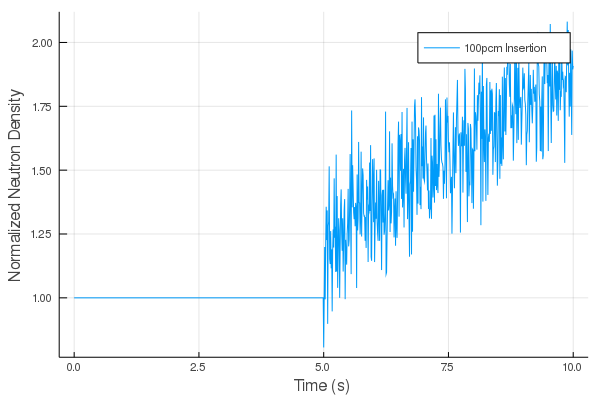
\includegraphics[width=0.5\textwidth]{../plots/analytical-sols/100pcm_fp_error.png}
  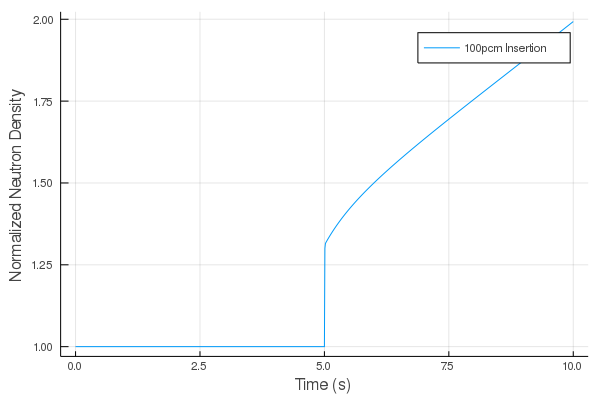
\includegraphics[width=0.5\textwidth]{../plots/analytical-sols/100pcm.png}
  \caption{Left: The analytical solution to the Point Kinetics equations under a $100$ pcm insertion
  as defined in Eq.~\cref{eq:analytical-step} with use of the native \texttt{Float64} precision.
  Right: The same solution, but instead with \texttt{Double64} (a $128$ bit floating point number)
  as the basis. The error is resolved, and the pertinent features are evident. The insertions occur
  at $t = 5$s. Note some important defintions for these types of transients. The steep rise
  at $t = 5$s is refered to as the ``prompt jump", after which, the delayed neutron generation
  catches up and we see a slower growth in reactor power.}
  \label{fig:single-double-prec}
\end{figure}

Additionally, we will examine reactivity insertions on the order of $1$\$, which
diverge very quickly. \cref{fig:dollar-insert-analytical} shows the analytical
solution to the point kinetics equations under a step insertion of $1$\$.\\

\begin{figure}[htb]
  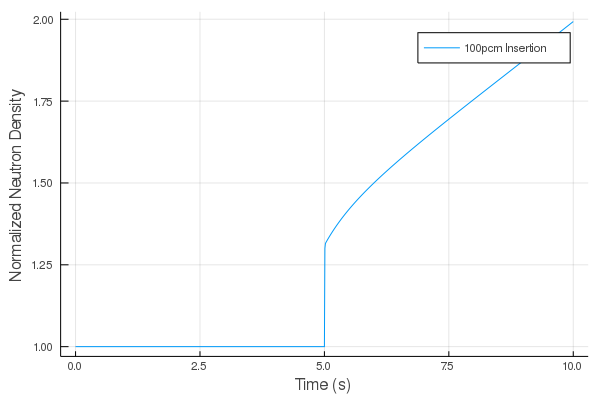
\includegraphics[width=0.5\textwidth]{../plots/analytical-sols/100pcm.png}
  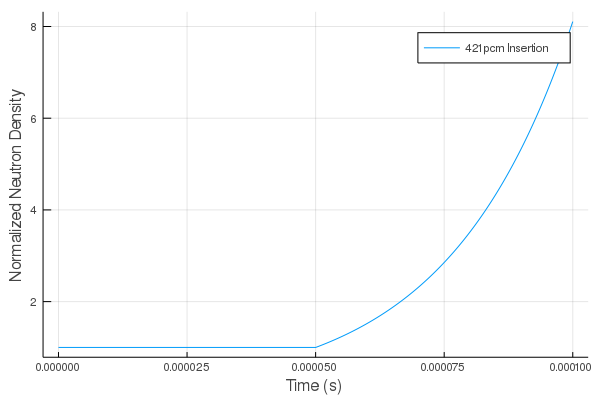
\includegraphics[width=0.5\textwidth]{../plots/analytical-sols/421pcm.png}
  \caption{Left: A reproduction of the right plot from \cref{fig:single-double-prec}.
  Right: The analytical solution defined in Eq.~\cref{eq:analytical-step} with a
  reactivity insertion of $1$\$ or $421$ pcm. Note that the prompt jump is so large that the
  solution diverges within a thousandth of a second. These two curves represent our
  test case solutions.}
  \label{fig:dollar-insert-analytical}
\end{figure}

These two curves are a baseline to which we compare all of our computed solutions,
giving a quantifiable metric for accuracy in both tranients.

\section{Solving the Point Kinetics Equations}

\subsection{Building an Optimal Derivative Defintion}
In order to perform any sort of reasonable benchmarking for solver algorithms,
we must ensure that our ODE definition is optimal, such that any discrepancies in
solution time are not drowned out by overhead. There are a few things we can check
to ensure optimality in our ODE definition: (1) memory allocations, and (2) type stability. \\

Using the \texttt{BenchmarkTools.jl} \texttt{@btime} and \texttt{@benchmark} macros,
we can demonstrate that our inner loop (the \texttt{pk!} method) has minimal allocations.
Particularly, we can achieve almost no (2) heap allocations per inner loop (a result of
our two \texttt{@view} macro calls), totalling only $96$ bytes. \\

Now we can use the type inferencing capabilities of \texttt{Julia}'s JIT compiler
to speed up our solves. To achieve type stability, we define an abstract type family,
\texttt{AbstractInsert}, that handles arbitraty reactivity insertion functions.
This allows the parameters used within the inner loop to be fully type stable.
The \texttt{@code\_warntype} macro shows no potential type
ambiguities throughout our inner loop, so we can be assured the JIT compiler is
producing optimal type inferences. \\

% Finally, we can use the \texttt{Profle.jl} module to corroborate the above two
% conclusions, that, our ODE definition is in fact optimal. This
% plot shows the relative time spent in each function called during the solve. Highlighted
% in \cref{fig:flame-plot} are sections of importance. In general, though,
% there is little overhead from the solver, so most of the computation time is spent
% doing the actual integration.\\
%
% \begin{figure}[htb]
%   % \includegraphics[width=0.5\textwidth]{../plots/flame-plots/100pcm_flame_plot.png}
%   \caption{}
%   \label{fig:flame-plot}
% \end{figure}

Now we can effectively dive into a solver analysis with the guarantee that algorithmic
differences in the integrators produce the variance in the total runtimes, and not
computational inefficiencies. Note that in the following sections, we define a
``branching" insertion as a step function with a jump discontinuity, while a
``smoothed" insertion is a hyperbolic tangent function of equal magnitude. Both
options are shown in \cref{fig:branch-smooth}

\begin{figure}[htb]
  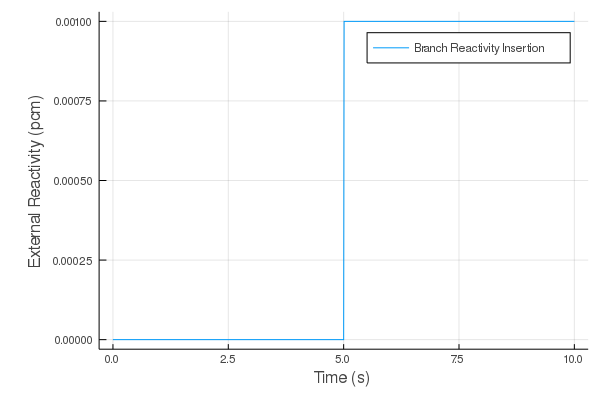
\includegraphics[width=0.5\textwidth]{../plots/insertion-plots/branch.png}
  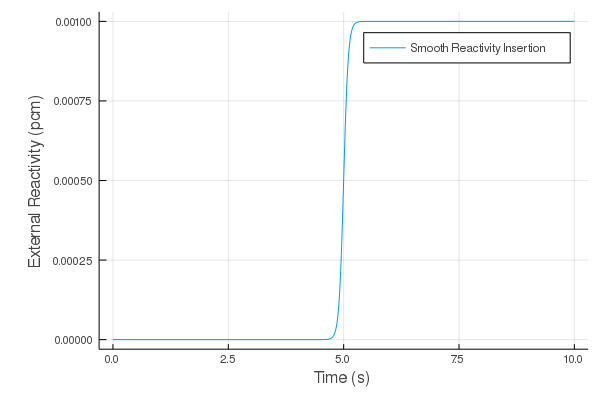
\includegraphics[width=0.5\textwidth]{../plots/insertion-plots/smooth.png}
  \caption{Left: a branched insertion of $100$ pcm. Right: a smoothed insertion of $100$ pcm. We
  use the hyperbolic tangent function with steepness $k=10$: $\frac{\rho}{2}(\tanh{(t - 5)k} + 1)$.}
  \label{fig:branch-smooth}
\end{figure}

\subsection{Metrics for Evaluating Integrator Performance}
In the following sections we present a detailed analysis of the efficacy of a litany of solvers
at a variety of tolerances. The best metric for rating the performace of a solver algorithm
is an open question. The objectives are user-specific, so for the sake of making a
conclusion, we specify our user needs here. We set out to create a high-speed,
reasonably accurate simulator to be used in core design work and reactor control
optimizations. There are a few key threshold criteria that we require of our simulator:\\

\begin{enumerate}
  \item Prioritize speed to within reasonable accuracy
  \item Resolve the prompt jump to high fidelity %($10^{-6}$ or better)
  \item Approximate netron densities during delayed effects to a decent accuracy, but less
  so than than the prompt jump %within $10^{-4}$
  \item Have the ability to accept a reactivity insertion of arbitrary shape
  % \item Outperform an existing Python implementation.
\end{enumerate}

It is with these demands in mind that we can evaluate each integration algorithm.\\

Note that for the following sections regarding solver performance, the computer
with specifications described in \cref{tab:computer-specs} is used.

\begin{table}[htb]
  \begin{center}
    \begin{tabular}{c|c}
      Intel i7-7700&4.2 GHz (8 Core)\\
      DDR4 2400 MHz&32 Gb\\
      GeForce GTX 1080ti&11.34 TFLOPS (Float32)\\
    \end{tabular}
  \end{center}
  \caption{Computer specifications for this performance analysis.}
  \label{tab:computer-specs}
\end{table}

\subsection{Solving a 100 pcm Step Insertion}

We approach the definition of a step insertion in two ways: (1) as a branched
function with a jump discontinuty, and (2) as a smooth hyperbolic tangent function
of equal size. For each of these two definitions of a step insertion, we
evaluate the solvers on three criteria: \\


\begin{enumerate}
  \item Total runtime
  \item Number of accepted and rejected steps
  \item Average and final timepoint error in neutron density\\
\end{enumerate}


Let's begin by examining our solver algorithms under a low tolerance for the $100$
pcm insertion. \cref{fig:low-tol-both} shows the work precision plots for
both the branching and smoothed insertions.

\begin{figure}[htb]
  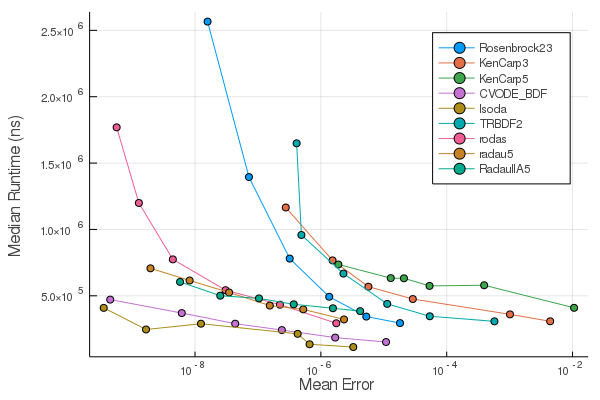
\includegraphics[width=0.5\textwidth]{../plots/work-precision/-low_tolerance_100pcm.png}
  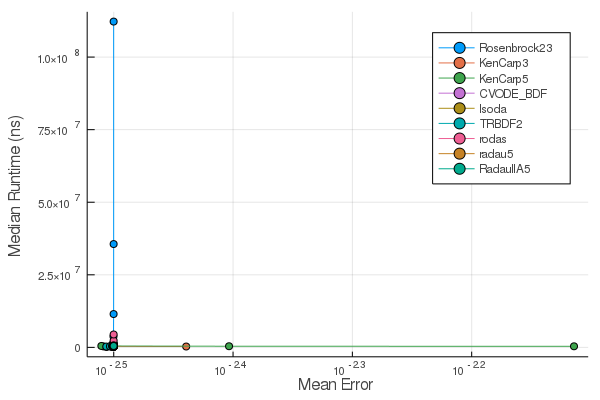
\includegraphics[width=0.5\textwidth]{../plots/work-precision/-low_tolerance_100pcm_tanh.png}
  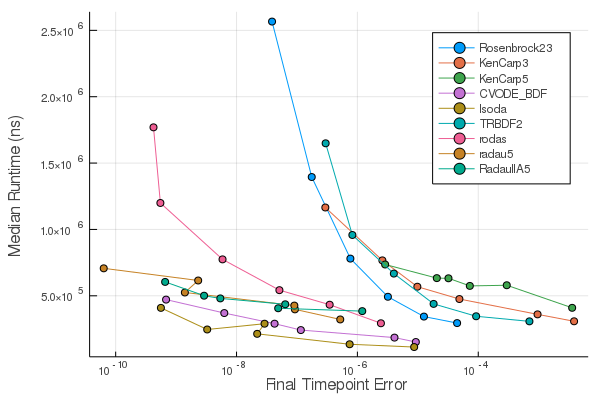
\includegraphics[width=0.5\textwidth]{../plots/work-precision/final_tp-low_tolerance_100pcm.png}
  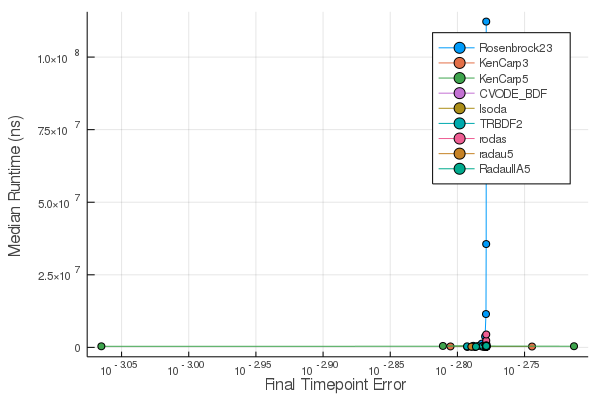
\includegraphics[width=0.5\textwidth]{../plots/work-precision/final_tp-low_tolerance_100pcm_tanh.png}
  \caption{Left: mean timeseries error and final timepoint error for a branching step insertion. Right: mean timseries error and final timepoint error for the hyperbolic tangent smoothed insertion. }
  \label{fig:low-tol-both}
\end{figure}

With low tolerances ($10^{-12} \rightarrow 10^{-7}$), we have a relatively clear
delineation of solver performance. The top two performing algorithms are LSODA and
CVODE\_BDF, both in terms of accuracy and runtime. The native \texttt{Julia} RadauIIA5
performs quite similarly to its counterpart RADAU5, which implies that the integration
is relatively agnostic to language implementation. The KenCarp methods are consistently
the worst performing of the set, and Rosenbrock23, while slightly slower, achieves higher
accuracy than its remaining \texttt{Julia} counterparts.\\

We see that the smoothed solutions are effectively
the same for all solvers in terms of accuracy. There are some notable exceptions:
both KenCarp methods produce higher variance in their solution accuracy. Rosenbrock23
handles the smoothed insertion much more poorly at low tolerances than do the remaining
algorithms. \\

Note that in both of these cases, DOPRI5 was analyzed as a potential ``worst-case"
Runge-Kutta method, and in fact, it performed so poorly, it has been omitted from these
plots. Now we can look into the performance of these solution algorithms in cases where
accuracy is of less importance. These results are compiled in \cref{fig:high-tol-both}.\\

\begin{figure}[htb]
  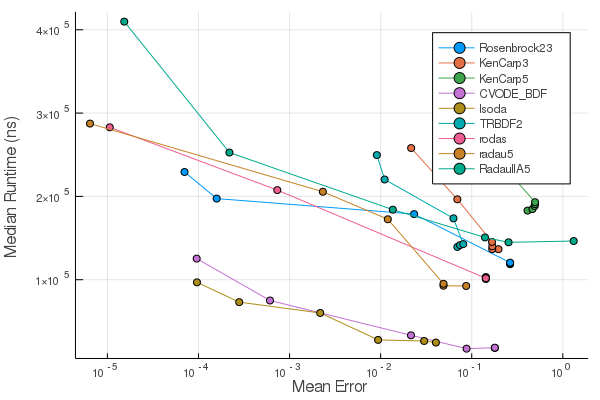
\includegraphics[width=0.5\textwidth]{../plots/work-precision/-high_tolerance_100pcm.png}
  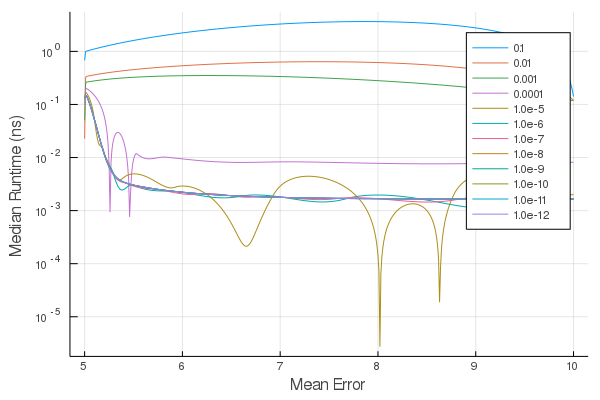
\includegraphics[width=0.5\textwidth]{../plots/work-precision/-high_tolerance_100pcm_tanh.png}
  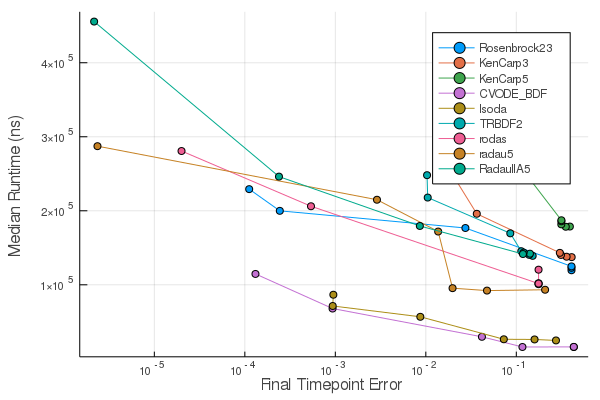
\includegraphics[width=0.5\textwidth]{../plots/work-precision/final_tp-high_tolerance_100pcm.png}
  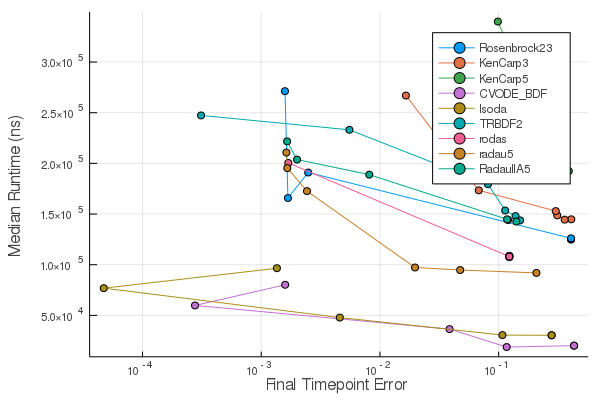
\includegraphics[width=0.5\textwidth]{../plots/work-precision/final_tp-high_tolerance_100pcm_tanh.png}
  \caption{Left: mean timeseries error and final timepoint error for a branching step insertion. Right: mean timseries error and final timepoint error for the hyperbolic tangent smoothed insertion. }
  \label{fig:high-tol-both}
\end{figure}

For higher tolerances ($10^{-6} \rightarrow 10^{-1}$), for our branched insertion,
we see similar trends to the
low tolerance cases, though with some variation in accuracy. Again, from a holistic
viewpoint, both LSODA and CVODE\_BDF seem to outperform all other solvers, particularly with
respect to their runtimes. However, RADAU5 and RadauIIA5 make a strong case for accuracy at higher
tolerances at the expence of a few 10ths of a millisecond per run. Once again, the KenCarp methods
and TRBDF2 perform quite poorly. The same can be said about the results from the smoothed
case, however with an overall reduction in average runtime across all solvers. \\

As a representative example, let's examine the time dependent error of one of the top
performing algorithms, CVODE\_BDF. \cref{fig:timeseries-error} shows the effect
that smoothing has on accuracy of a critical part of the solution.\\

\begin{figure}[htb]
  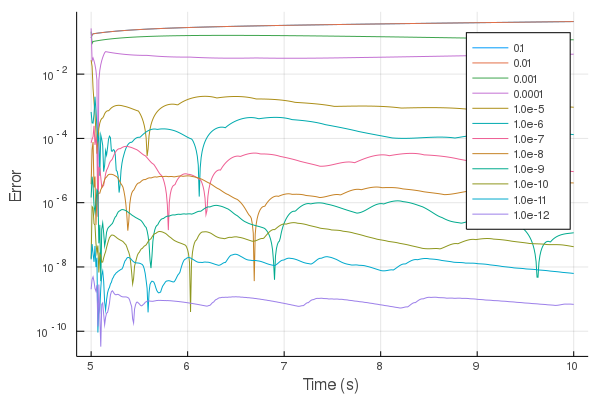
\includegraphics[width=0.5\textwidth]{../plots/timeseries-error/CVODE_BDF.png}
  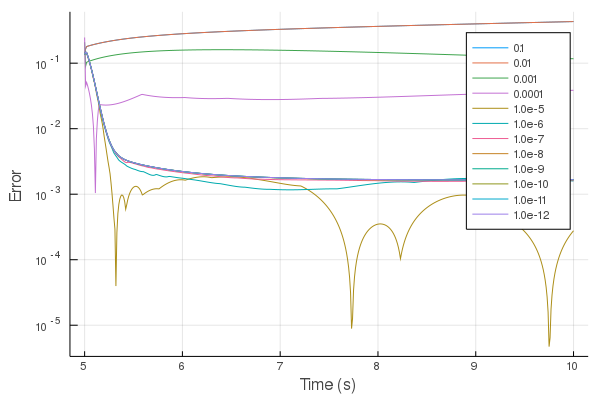
\includegraphics[width=0.5\textwidth]{../plots/timeseries-error/CVODE_BDF-tanh.png}
  \caption{Left: error as a function of time for CVODE\_BDF with branched insertion.
  Right: error as a function of time for same algorithm but with smoothed insertion. Both
  plots begin at the time of insertion.}
  \label{fig:timeseries-error}
\end{figure}

As is shown in \cref{fig:timeseries-error}, there is a considerable difference in
the magnitudes of the accuracy after the smoothing of the reactivity insertion.
What is particularly troublesome is the error during the first $\sim 0.1$s of the
insertion. Accuracy in defining the shape of the prompt jump is important. Afterwards,
the error in the delayed neutron propagation is less critical. While this distinction
may be enough to sway a user with a need of higher accuracy, for the purposes of
approximating reactor dynamics for use in quick iterative engineering tasks, smoothing
is feasible. Should we deem the reduction in accuracy due to smoothing acceptable,
we can see how much more performant the solvers are in those cases.\\

In addition to tracking total runtime, we have also recorded the number of solve
iterations each algorithm takes. These results are compiled for all tolerances for
each solver in \cref{fig:num-steps}. \\

\begin{figure}[htb]
  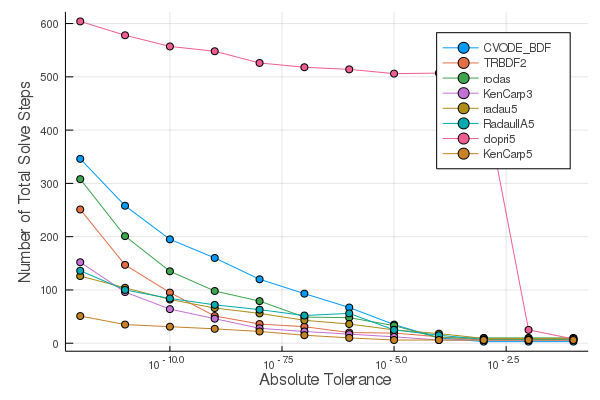
\includegraphics[width=0.5\textwidth]{../plots/step-plots/stepinsert.png}
  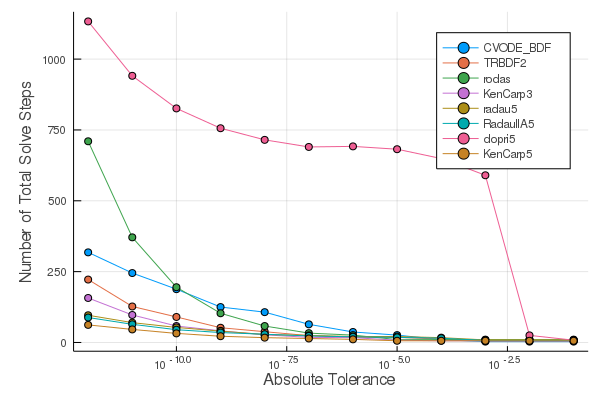
\includegraphics[width=0.5\textwidth]{../plots/step-plots/tanhinserts.png}
  \caption{Left: number of steps required to solve Point Kinetics equations with
  branching insertion. Right: number of steps required to solve with a smoothed
  insertion. Note that Rosenbrock23 took far too many steps in the smoothed case
  to warrant plotting, and that LSODA does not support the counting of steps during
  its solve.}
  \label{fig:num-steps}
\end{figure}

Here we have some interesting results. There are a few algorithms whose number of
steps worsens through smoothing (particularly our regular poor performers Rosenbrock23
and DOPRI5). More importantly, though, our faster algorithms such as CVODE\_BDF and
RADAU5/RadauIIA5 drastically decrease in the number of steps required and therefore
the required runtime.

\subsection{Solving a 421pcm Insertion}
A $421$ pcm insertion corresponds to exactly $1$\$ for the described reactor.
While not a transient expected for any sort of normal transient through which the
assumptions made by the Point Reactor model would survive for more than a few microseconds,
this transient is a industry classic for evaluating solver performance. This transient
is benchmarked as a prompt criticality test. \\

Let's begin by examining the high tolerance region again ($10^{-6} \rightarrow 10^{-1}$).
The results are compiled in \cref{fig:high-tol-both-dollar}.
\begin{figure}
  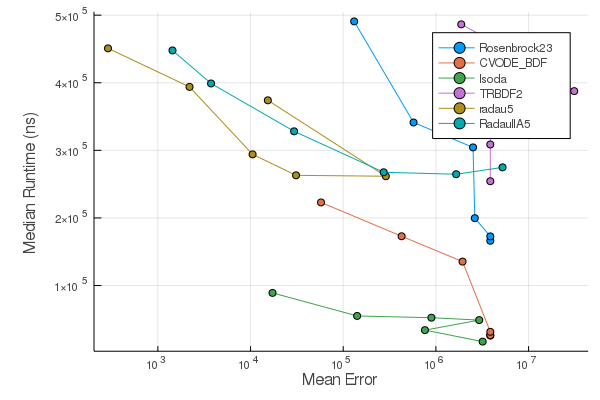
\includegraphics[width=0.5\textwidth]{../plots/work-precision/-high_tolerance_421pcm.png}
  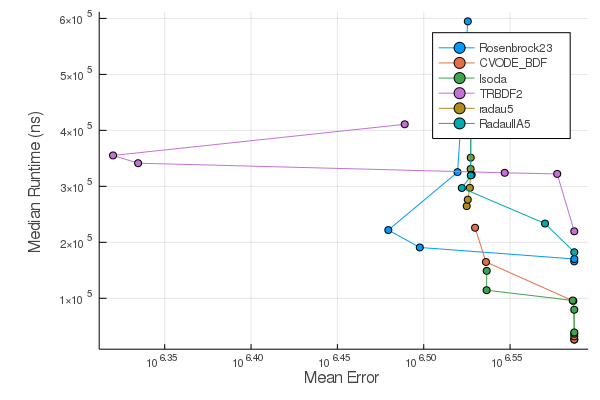
\includegraphics[width=0.5\textwidth]{../plots/work-precision/-high_tolerance_421pcm_tanh.png}
  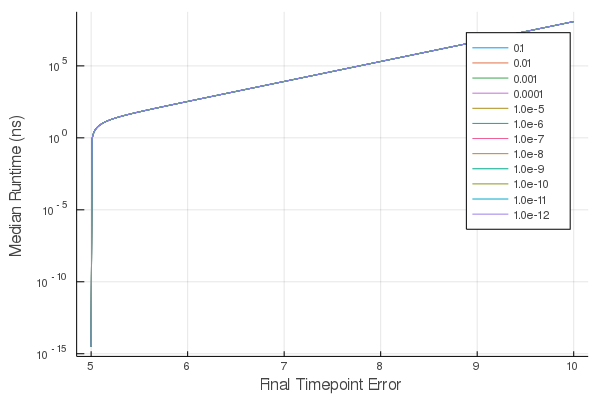
\includegraphics[width=0.5\textwidth]{../plots/work-precision/final_tp-high_tolerance_421pcm.png}
  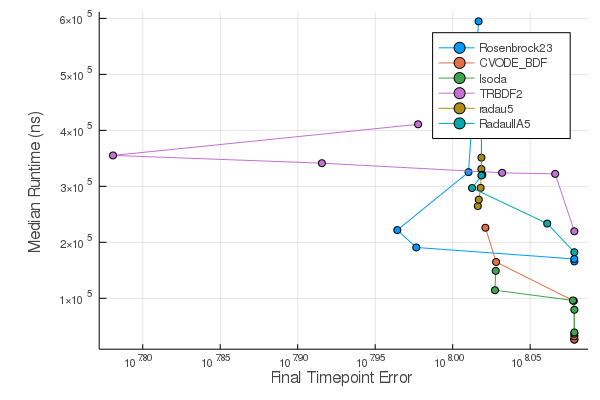
\includegraphics[width=0.5\textwidth]{../plots/work-precision/final_tp-high_tolerance_421pcm_tanh.png}
  \caption{Left: branched insertion of $1$\$ reactivity with high tolerances.
  Right: smoothed insertion of $1$\$ with high tolerances}
  \label{fig:high-tol-both-dollar}
\end{figure}
Here, it is clear that the looseness in our rolerance settings has allowed for
an error that makes these solutions unusable. The final timepoint of the analytical
solution under the dollar insertion is on the order of $10^8$, and these solutions
(with the exception of a few more accurate performers like RADAU5 and RadauIIA5)
have error of roughly that size. It would be ludicrous to draw conclusions about
relative solver performance in a scenario in which no solver produced meaningful
results. So, let's move on to the low tolerance regime. \\

For lower tolerances ($10^{-12} \rightarrow 10^{-7}$), we see much different results.
The work precision diagrams for these tolerances are compiled in \cref{fig:low-tol-both-dollar}.
\begin{figure}
  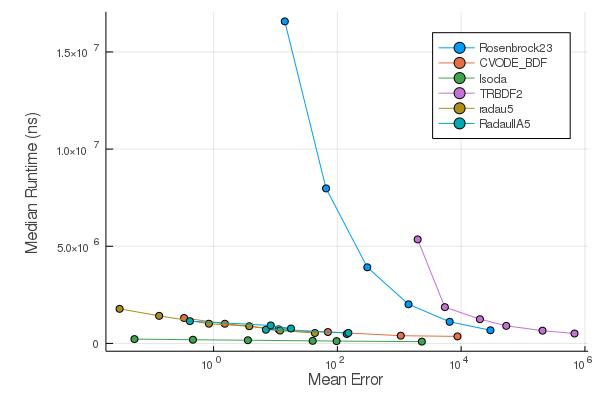
\includegraphics[width=0.5\textwidth]{../plots/work-precision/-low_tolerance_421pcm.png}
  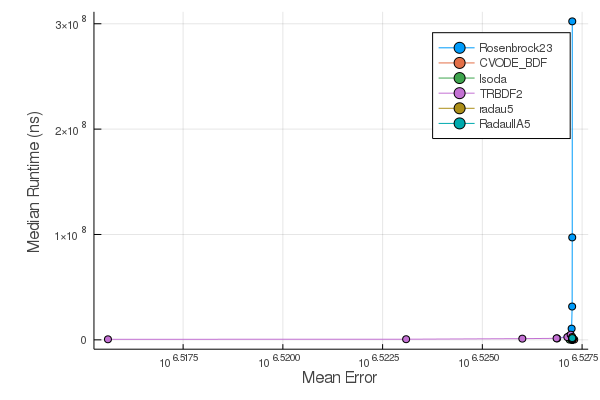
\includegraphics[width=0.5\textwidth]{../plots/work-precision/-low_tolerance_421pcm_tanh.png}
  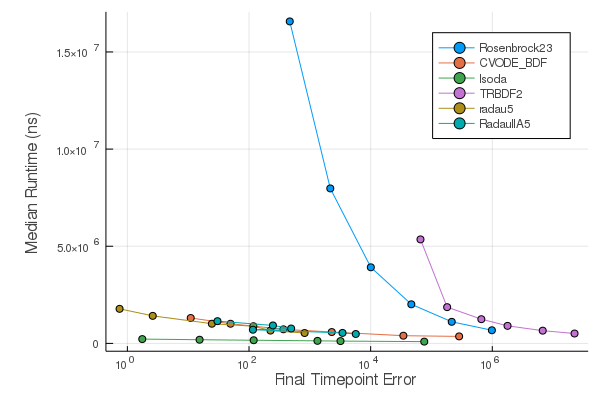
\includegraphics[width=0.5\textwidth]{../plots/work-precision/final_tp-low_tolerance_421pcm.png}
  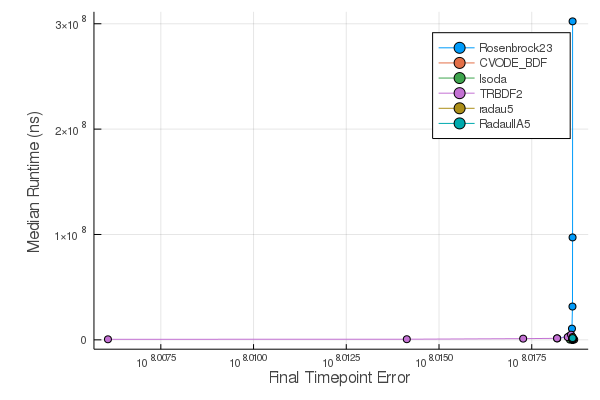
\includegraphics[width=0.5\textwidth]{../plots/work-precision/final_tp-low_tolerance_421pcm_tanh.png}
  \caption{Left: branched insertion of $1$\$ reactivity with low tolerances.
  Right: smoothed insertion of $1$\$ with low tolerances}
  \label{fig:low-tol-both-dollar}
\end{figure}
Right away, we can exclude our smoothed insertion results. All solvers essentially performed
the same, and with very high error, and no time improvement over the branched input.
The volatile nature of this transient is such that smoothing introduced far too much
error to the solution. This likely increased runtimes the smoothing enlarged the duration
of the insertion, meaning the solvers were under small timestepping constraints for
much longer, drowning out any of the improvements we see in the $100$ pcm case. \\

For the branched input, however, we see great results out of our consistent top
performers. LSODA, CVODE\_BDF, RADAU5, and RadauIIA5 reach errors below $10^2$,
the best of which (RADAU5) gets to about $10^-1$ ($\sim 0.7$ final timepoint
error to be exact). While these algorithms were not designed for high accuracy in the
extreme cases of the Point Kinetics equations, these results do give much credence
to their accuracy under high volatility. There are existing algorithms, such as the
special case of Backwards Euler created by Barry Ganopol (colloquially referred to as
the ``neutron transport cowboy" in the nuclear industry)
that are the gold standard for highly accurate results under these
large insertions. \cite{Ganopol_accurate} Nonetheless, for the purposes of handling
a wide variety of transients the top algorithms described in this analysis are
perfect for fast, iterative reactor design.

\section{Conclusions}
The objective of this analysis was threefold: (1) develop an optimal \texttt{Julia}
Point Kinetics simulator, (2) analyze the performance of various native and non-native
solution algorithms on a particular reactor transient, and (3) prescribe an algorithm
for use in reactor engineering. To these ends we can conclude the following with respect
to the step insertion test case. In all $100$ pcm cases, non-native solvers such as LSODA and
CVODE\_BDF outperformed the native \texttt{Julia} implementations, which goes
against the conventional wisdom that the native algorithms perform well on smaller
ODEs. Additionally, when the step insertion is smoothed, we see a drastic reduction in the number of adaptive
steps required for \emph{most} solvers (those that increase were ill fit to solve the
branched case anyway). Finally, in the interest of qualifying these solution algorithms
against the peak of the nuclear academic community, we completed an analysis of the $1$\$
insertion case. While their performance does not match that of the top-shelf methods
used in academia for $1$\$ insertions, these algorithms showed enough accuracy under the
most extreme cases to warrant their use in iterative reactor design models.

\section*{Acknowledgments}
A big thank you to Dr. Chris Rackauckas for his incredible help in shaping and debugging
this analysis.

\bibliographystyle{siamplain}
\bibliography{references}
\end{document}
